\section{Actividad 1}
Presento la estructura del presente laboratorio:
  \centering
  \includegraphics[width=0.5\textwidth]{img/Screenshot_2023-10-16-14-45-28_1920x1080.png}
\section{Actividad 2 y 3}
    \begin{itemize}
        \item Para esta actividad de creo la clase soldado con los siguientes atributos
    \end{itemize}
\begin{lstlisting}[language=java, caption={Clase Soldado.java}]
public class Soldado{
  public String name;
  public int life;
  public int row;
  public int column;

  public Soldado(String name){
    this.name = name;
  }
}
\end{lstlisting}
\begin{itemize}
    \item Cada uno de los atributos tiene sus apropiados metodos setters y getters
    \item La actividad 4 en realidad solo es una especificacion asi que continuemos con la actividad 5
\end{itemize}
\section{Actividad 5}
\begin{itemize}
    \item Se modifico el codigo de videojuego.java del laboratorio 3, para hacer que la inicializacion dejercitos nos de como resultado un ejercito de entre 1 y 10 soldados
    \item Para esto usamos la clase Random 
    \end{itemize}
    \begin{lstlisting}[language=java, caption={Clase Videojuego.java}]
  public static Soldado[] initializeArmy(){
    Random rand = new Random();
    int randNum = rand.nextInt(10) + 1;
    Soldado[] army = new Soldado[randNum];

    for(int i = 0; i < randNum; i++){
      army[i] = new Soldado("Soldado " + (i + 1));
    }
    return army;
  }
\end{lstlisting}
\begin{itemize}
    \item Ahora agregaremos la funcionalidad de que cada soldado se genere con un nivel de vida de entre 1 y 5
\end{itemize}

    \begin{lstlisting}[language=java, caption={Clase Videojuego.java}]
  public static Soldado[] initializeArmy(){
    Random rand = new Random();
    int randNum = rand.nextInt(10) + 1;
    Soldado[] army = new Soldado[randNum];

    for(int i = 0; i < randNum; i++){
      army[i] = new Soldado("Soldado " + (i + 1));
      army[i].setLife(rand.nextInt(5) + 1);
    }
    
\end{lstlisting}

Ahora, para graficar a los soldados usaremos una biblioteca que fue desarrollada el semestre pasado en Fundamentos de la Programacion 1.
 Esta biblioteca es graphics, que puede mostrar un grafico de un tablero de ajedrez por pantalla, para mostrar a los soldados se creo un nuevo tipo de figura (soldier)

 Esta es la estructura de la biblioteca graphics:

  \centering
  \includegraphics[width=0.5\textwidth]{img/treeGraphics.png}

  \begin{itemize}
      \item Lo que se hizo a continuacion es un metodo que grafique el estado actual del tablero, usando graphics
  \end{itemize}
      \begin{lstlisting}[language=java, caption={Clase Videojuego.java}]
  public static void makeGBoard(){
    for(int i = 0; i < 10; i++){
      Picture fila = null;
      for(int j = 0; j < 10; j++){
        Picture c = Picture.casilleroBlanco();
        if(board[i][j] != null)
          c = Picture.soldier().superponer(c);
        if(j == 0){
          fila = c;
          continue;
        }
        fila = fila.alLado(c);
      }
      if(i == 0){
        gBoard = fila;
        continue;
      }
      gBoard = gBoard.encima(fila);
    } 
  } 
\end{lstlisting}
\begin{itemize}
    \item Se recorre por filas y columnas sobre los elementos de nuestro ejercito de soldados, y en caso de encontrar a un soldado en alguna posicion (boardi[i][j] != null) imprime un soldado en esa posicion y la manda a una fila general que la mandara a su vez a un tablero (gBoard)
    \item Al final del metodo tendremos el tablero gBoard con los soldados en las posiciones requeridas
\end{itemize}

\subsection{Mostrando los datos por pantalla}
\begin{itemize}
    \item Ahora que tenemos todo lo necesario para correr el juego, necesitamos metodos para mostrar todo lo que hemos trabajado
    \item Tenemos 3 display's, mostrar un soldado, un ejercito, y el tablero, veamos el primero:
\end{itemize}
\subsubsection{Mostrar soldado}
      \begin{lstlisting}[language=java, caption={Clase Videojuego.java}]
  public static void displaySoldier(Soldado s){
    System.out.println(" " + s.getName() + ":");
    System.out.println("  Nivel de vida: " + s.getLife());
    System.out.println("  Fila: " + (s.getRow() + 1));
    System.out.println("  Columna: " + (s.getColumn() + 1));
    System.out.print("\n");
  }
\end{lstlisting}
\begin{itemize}
    \item Como vemos, el metodo recibe un soldado, y luego muestra datos como la vida, el nombre, la fila en la que se ubica y la columna en la que esta
    \item Este metodo nos vservira por que lo usaremos despues en el metodo de mostrar ejercito y tambien para mostrar al soldado con mayor puntaje de vida
\end{itemize}
\subsubsection{Mostrar un ejercito}
      \begin{lstlisting}[language=java, caption={Clase Videojuego.java}]
  public static void displayArmy(Soldado[] army){
    System.out.println("\n===== Army Soldiers =====");
    for(Soldado soldier : army){
      displaySoldier(soldier);
    }
  }
\end{lstlisting}
\begin{itemize}
    \item La entrada que recibe el metodo es un ejercito de soldados
    \item El metodo recorre el ejercito entero
    \item En cada vuelta, hace una lolamada al metodo que desarrollamos antes
\end{itemize}
\subsubsection{Mostrando el tablero en pantalla}
\begin{itemize}
    \item Quiza esto es un poco mas facil
    \item Usamos la clase Graphics de la biblioteca graphics, para imprimir en una ventana emergente el tablero que ya creamos con anterioridad:
\end{itemize}
      \begin{lstlisting}[language=java, caption={Clase Videojuego.java}]
  public static void displayBoard(){
    Graphics g = new Graphics(gBoard);
    g.print();
  }
\end{lstlisting}
\subsubsection{Ejecucion}
\begin{itemize}
    \item La ejecucion de esta porcion de codigo esta dividida en dos partes
    \item La primera parte es la parte grafica, el tablero se dibuja en la pantalla y muestra a los soldados que han sido creados
    \item La segunda parte es la ista en consola, que muestra los datos de los sondados que han sido creados
    \item Adicionalmente se pide el soldado con mas vidas, y el promedio de vidas
    \item Esto lo lograremos poniendo contadores que recopilen datos y usamos los metodos de display para mostrarlos en pantalla:
\end{itemize}
  \centering
  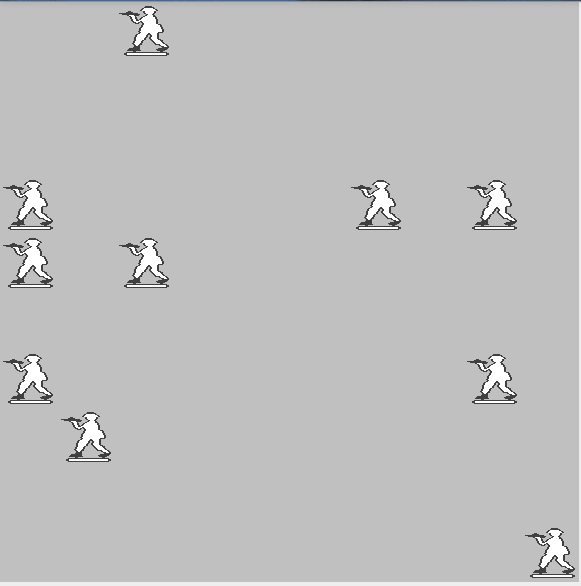
\includegraphics[width=0.5\textwidth]{img/ejecucion1.png}
  \begin{itemize}
      \item Ahora veremos los datos mostrados por consola:
      
  \end{itemize}
        \begin{lstlisting}[language=java, caption={Consola}]
===== Army Soldiers =====
 Soldado 1:
  Nivel de vida: 5
  Fila: 4
  Columna: 9

 Soldado 2:
  Nivel de vida: 5
  Fila: 4
  Columna: 7

 Soldado 3:
  Nivel de vida: 5
  Fila: 1
  Columna: 3

 Soldado 4:
  Nivel de vida: 4
  Fila: 4
  Columna: 1

 Soldado 5:
  Nivel de vida: 2
  Fila: 10
  Columna: 10

 Soldado 6:
  Nivel de vida: 5
  Fila: 5
  Columna: 1

 Soldado 7:
  Nivel de vida: 5
  Fila: 7
  Columna: 1

 Soldado 8:
  Nivel de vida: 3
  Fila: 7
  Columna: 9

 Soldado 9:
  Nivel de vida: 5
  Fila: 8
  Columna: 2

 Soldado 10:
  Nivel de vida: 1
  Fila: 5
  Columna: 3

Soldado con maxima vida:
 Soldado 1:
  Nivel de vida: 5
  Fila: 4
  Columna: 9
\end{lstlisting}

\subsection{Orednamiento por vida}
\begin{itemize}
    \item Para hacer el ordenamiento de los soldados por dos metodos de ordenamiento, lo haremos por buble sort y por insertion sort
    \item Como se nos dio la indicacion que podemos reutilizar el codigo de los laboratorios 3 y 4, usaremos la implementacion de algoritmos de ordenamiento del laboratorio 4
    \item Con esta gran ayuda, la  implementacion de ordenamiento por vida se reduce a reemplazar el nombre de las variables y clases usadas
\end{itemize}
\subsubsection{Bubble sort}
\begin{itemize}
    \item Costa de dos metodos, el ordenamiento es una implementacion del algoritmo buble sort
    \item El metodo auxiliar para intercambiar dos elementos de un ejercito
\end{itemize}


      \begin{lstlisting}[language=java, caption={Metodo auxiliar}]
  public static void intercambiar(Soldado[] army, int i, int j){
    Soldado aux = army[i];
    army[i] = army[j];
    army[j] = aux;
  }
\end{lstlisting}
      \begin{lstlisting}[language=java, caption={Metodo bubble sort}]
  public static void bubbleSortLife(Soldado[] army){
    for(int i = 0; i < army.length - i; i++){
      for(int j = 0; j < army.length - 1 - i; j++){
        if(army[j].getLife() > army[j + 1].getLife())
          intercambiar(army, j, j + 1);
      }
    }
  }
\end{lstlisting}

\subsubsection{Insertion sort}
\begin{itemize}
    \item El metodo de ordenamiento por vida usando el algoritmo de insertion sort solo consta de un metodo principal
\end{itemize}
      \begin{lstlisting}[language=java, caption={Metodo bubble sort}]
  public static void insertionSortLife(Soldado[] army){
    for(int i = 1; i < army.length; i++){
      Soldado actual = army[i];
      int j = i - 1;
      while(j >= 0 && army[j].getLife() > actual.getLife()){
        army[j + 1] = army[j];
        j--;
      }
      army[j + 1] = actual;
    }
  }
\end{lstlisting}


\section{Commits}
\begin{itemize}
    \item Estuve investigando sobre buenas practicas de redaccion de commits y encontre las 7 reglas de los mensajes de commits
    \item Estas reglas fueorn aplicadas en cada uno de los commits
    \item De manera que no es necesario hacer una explicacion a detalle de cada uno, ya que la explicacion la contiene el mismo mensaje de commit
    \item A continuacion muestro los commits principales:
\end{itemize}
      \begin{lstlisting}[language=bash, caption={Commits principales}]
commit d11009b95725f37e26823da21d9479c457c44c70
Author: JhonatanDczel <jariasq@unsa.edu.pe>
Date:   Thu Oct 12 15:10:27 2023 -0500

    Crear el proyecto laboratorio 05

    Agregar el documento de enunciado y crear la estructura de
    archivos para el trabajo
\end{lstlisting}
      \begin{lstlisting}[language=bash, caption={Commits principales}]
commit f1ef7a39016c465a391cce3804443090edc9cc94
Author: JhonatanDczel <jariasq@unsa.edu.pe>
Date:   Mon Oct 16 09:24:41 2023 -0500

    Completa la actividad 2

    Se creo la clase soldado.java con las especificaciones requeridas de
    atributos y metodos
\end{lstlisting}
      \begin{lstlisting}[language=bash, caption={Commits principales}]
commit 5a4c515463e334555acd69dadea0b3bfb40d321d
Author: JhonatanDczel <jariasq@unsa.edu.pe>
Date:   Mon Oct 16 09:34:44 2023 -0500

    Avanza la actividad 5

    Se puso el sistema para que el soldado reciba una cantidad de vida
    aleatoriamente entre 1 y 5
\end{lstlisting}
      \begin{lstlisting}[language=bash, caption={Commits principales}]
commit d53d0fb5620edef79329eb845833aea3df29641d
Author: JhonatanDczel <jariasq@unsa.edu.pe>
Date:   Mon Oct 16 10:11:06 2023 -0500

    actividad 5: biblioteca para graficar el tablero

    Se agrego la biblioteca graphics.jar que hicimos en Fundamentos 1, para
    graficar el tablero con los soldados representados por peones
\end{lstlisting}

      \begin{lstlisting}[language=bash, caption={Commits principales}]
commit 21c0de14822b4271d21dc2df144d7626f7398eb1
Author: JhonatanDczel <jariasq@unsa.edu.pe>
Date:   Mon Oct 16 13:17:11 2023 -0500

    Modificar Picture para mostrar soldados

    Mosifique el codigo de la biblioteca graphics para generar en pantalla
    un soldado
\end{lstlisting}
      \begin{lstlisting}[language=bash, caption={Commits principales}]
commit 686cc633b17c5967511b97dc8ef0d311adf6d12a
Author: JhonatanDczel <jariasq@unsa.edu.pe>
Date:   Mon Oct 16 13:38:43 2023 -0500

    Crea el etodo displayBoard

    este metodo agarra el tablero (gBoard) y abre una ventana con la
    representacion grafica del estado actual
\end{lstlisting}
      \begin{lstlisting}[language=bash, caption={Commits principales}]
commit d162a8925fe59ea70ed1102a2c765a9f4bdd78ad
Author: JhonatanDczel <jariasq@unsa.edu.pe>
Date:   Mon Oct 16 13:50:32 2023 -0500

    Agrega el prototipo para calcular la vida promedio

    Se agrego codigo para recabar datos en la inicializacion de los
    ejercitos, luego dividirlos entre el total de soldados y finalmente
    guardarlos en una variable que contiene el promedio de vida de los ejercito
\end{lstlisting}
      \begin{lstlisting}[language=bash, caption={Commits principales}]
commit 7a9b21503e5bb29321cf14cf63e80a516022a664
Author: JhonatanDczel <jariasq@unsa.edu.pe>
Date:   Mon Oct 16 13:58:11 2023 -0500

    Reconoce al soldado de mayor vida

    En la inicializacion de ejercitos, se agrega codigo para comparar los
    nuevos soldados que van siendo creados con el soldado actual con mayor
    vida, en caso de que uno de ellos tenga mas vidas que este, se convierte
    en el nuevo soldado con mayor vida
\end{lstlisting}
      \begin{lstlisting}[language=bash, caption={Commits principales}]
commit 91add39b83886415a2102efd661401efd5290e83
Author: JhonatanDczel <jariasq@unsa.edu.pe>
Date:   Mon Oct 16 14:18:59 2023 -0500

    Implementa el metodo de ordenamiento bubble

    Se Agregan dos metodos, uno auxiliar para intercambiar dos soldados, y
    otro que es el metodo de ordenamiento por burbuja, usanco como base de
    comparacion la vida de los soldado
\end{lstlisting}
      \begin{lstlisting}[language=bash, caption={Commits principales}]
commit 741839fff18cd3d15c9dad5557c6fef0c10eec71 (HEAD -> main, origin/main)
Author: JhonatanDczel <jariasq@unsa.edu.pe>
Date:   Mon Oct 16 14:29:38 2023 -0500

    Implementa el ordenamiento de vida por insertion

    Se agrega un metodo que ordena a llos soldados por su vida
\end{lstlisting}
\section{Anexo: graphics y soldado}
Para lograr representar un soldado en pantalla se uso arte ascii para representar pixeles de distintos colores, en este caso se usaron los simbolos "hashtag" para el negro y "." para el blanco
\begin{itemize}
    \item El soldado tiene 58x58 en caracteres
    \item Se hizo representado con una fuente monoespaciada para no perder proporcion
    \item Para soldados de diferentes colores se puede invertir los simbolos usados
\end{itemize}
\newpage
      \begin{lstlisting}[language=java, caption={Representacion en ascii del soldado}]
	public static Picture soldier(){
		String [] img = {
          "                                                          ",
          "                                                          ",
          "                                                          ",
          "                                                          ",
          "                              #######                     ",
          "                             ##########                   ",
          "                           ##.........##                  ",
          "                          ##............##                ",
          "                         ##..............##               ",
          "             ###            ##.........##                 ",
          "           #######          ##.........##                 ",
          "    ###################      ##.......##                  ",
          "       ##################      ##....##                   ",
          "            ##.....#####      ##......##                  ",
          "              ##....#       ##........###                 ",
          "               ##...##    ##............##                ",
          "               ##...##   ##.............##                ",
          "                ##...## ##...............##               ",
          "                ##...###.................##               ",
          "                 ##......##..............##               ",
          "                  ###..## ##.............##               ",
          "                    ####   ##............##               ",
          "                           ##..............###            ",
          "                          ##.................##           ",
          "                          ##.................##           ",
          "                         ##...................##          ",
          "                        ##....................##          ",
          "                        ##.....................##         ",
          "                        ##.....................##         ",
          "                       ##......................##         ",
          "                        ##.................#####          ",
          "                       ##........##.......##              ",
          "                     ##.........####......##              ",
          "                    ##.........##  ##.....##              ",
          "                    ##.........##  ##.....##              ",
          "                   ##.........##  ##......##              ",
          "                   ##........##   ##......##              ",
          "                   ##........##    ##......###            ",
          "                   ##......##       ##.......###          ",
          "                  ##......##         ##.......##          ",
          "                  ##......##          ##.......##         ",
          "                 ##......##            ##.......##        ",
          "                  ##....###             #####.....##      ",
          "                   ##..##                   ##.....##     ",
          "                   ######                     ###...##    ",
          "                  #######                      #######    ",
          "              ###########                  ##########     ",
          "             ############                ###########      ",
          "            ##############                ########        ",
          "                  ###                        ###          ",
          "           #########################################      ",
          "         ###.......................................###    ",
          "         ###.......................................###    ",
          "           #########################################      ",
          "                                                          ",
          "                                                          ",
          "                                                          ",
          "                                                          "		
		};
		return new Picture(img);
	}
\end{lstlisting}
